%:
\documentclass[11pt]{article}


\usepackage{caption}

\usepackage{kotex}
\usepackage{sectsty}
\usepackage{graphicx}
\usepackage{amsmath}
\usepackage{amssymb}
\usepackage[margin=20mm]{geometry}
\usepackage{listings}
\usepackage{color}
\usepackage{lmodern} % Use a slightly nicer looking font
\usepackage{url} % Proper formatting for URLs
\usepackage{graphicx} % Handle inclusion of non-PDF graphics
\usepackage{subfig} % Allow sub-figures inside a figurexz
\usepackage{enumitem} % Allow lists to pick up numbering where the last list left off
\usepackage[margin=20mm]{geometry}
\usepackage{listings}
\usepackage{color}

\usepackage{setspace}
\usepackage{indentfirst}\setlength\parindent{2em}
\setstretch{1.5} %간격 맞추는 패키지


% Color definitions for source code listings
\definecolor{mygreen}{rgb}{0,0.6,0}
\definecolor{mygray}{rgb}{0.5,0.5,0.5}
\definecolor{mymauve}{rgb}{0.58,0,0.82}

\lstset{ 
  backgroundcolor=\color{white},   % choose the background color; you must add \usepackage{color} or \usepackage{xcolor}
  basicstyle=\footnotesize,        % the size of the fonts that are used for the code
  breakatwhitespace=false,         % sets if automatic breaks should only happen at whitespace
  breaklines=true,                 % sets automatic line breaking
  captionpos=b,                    % sets the caption-position to bottom
  commentstyle=\color{mygreen},    % comment style
  deletekeywords={...},            % if you want to delete keywords from the given language
  escapeinside={\%*}{*)},          % if you want to add LaTeX within your code
  extendedchars=true,              % lets you use non-ASCII characters; for 8-bits encodings only, does not work with UTF-8
  frame=single,	                   % adds a frame around the code
  keepspaces=true,                 % keeps spaces in text, useful for keeping indentation of code (possibly needs columns=flexible)
  keywordstyle=\color{blue},       % keyword style
  otherkeywords={*,...},           % if you want to add more keywords to the set
  numbers=left,                    % where to put the line-numbers; possible values are (none, left, right)
  numbersep=5pt,                   % how far the line-numbers are from the code
  numberstyle=\tiny\color{mygray}, % the style that is used for the line-numbers
  rulecolor=\color{black},         % if not set, the frame-color may be changed on line-breaks within not-black text (e.g. comments (green here))
  showspaces=false,                % show spaces everywhere adding particular underscores; it overrides 'showstringspaces'
  showstringspaces=false,          % underline spaces within strings only
  showtabs=false,                  % show tabs within strings adding particular underscores
  stepnumber=2,                    % the step between two line-numbers. If it's 1, each line will be numbered
  stringstyle=\color{mymauve},     % string literal style
  tabsize=2,	                   % sets default tabsize to 2 spaces
  title=\lstname                   % show the filename of files included with \lstinputlisting; also try caption instead of title
}


% Margins
\topmargin=-0.45in
\evensidemargin=0in
\oddsidemargin=0in
\textwidth=6.5in
\textheight=9.0in
\headsep=0.25in


\title{Linear Algebra \& Eigensystems Homework 4}
\author{MinWook Kang}
\date{\today}

\begin{document}
\maketitle
\pagebreak

% Optional TOC
% \tableofcontents
% \pagebreak


%--Paper--

\section{Linear Algebra}
\subsection{Introduction} 
선형 대수학은 모든 수학 분야의 중심이다. 
\begin{itemize}
    \item 선, 평면 및 회전과 같은 기본 물체를 정의하는 것을 포함하여 현대 기하학의 기본이다.
    \item 수학적 분석의 한 분야인 기능 분석은 함수 공간에 선형대수학을 적용하는 것을 볼 수 있다.
\end{itemize}
우리가 이번 섹션에 다뤄볼 것은 바로 선형 대수 방정식 세트에서 모르는  미지수를 푸는 것이다.

\begin{equation}
\begin{split}
\begin{aligned}
a_{00}x_0 + a_{01}x_1 + a_{02}x_2 + \cdots + a_{0,N-1}x_{N-1} &= b_0 \\
a_{10}x_0 + a_{11}x_1 + a_{12}x_2 + \cdots + a_{1,N-1}x_{N-1} &= b_1 \\
a_{20}x_0 + a_{21}x_1 + a_{22}x_2 + \cdots + a_{2,N-1}x_{N-1} &= b_2 \\
                                                              &\cdots \\
a_{M-1,0}x_0 + a_{M-1,1}x_1 + a_{M-1,2}x_2 + \cdots + a_{M-1,N-1}x_{N-1} &= b_{M-1} \\
\end{aligned}
\end{split}
\end{equation}


N이 주어졌을때,  모르는 $x_{j}$에 대해서 M개의 방정식이 연관된다. 계수 $a_{ij}$에서 $i =.0,1,...,M-1$을 만족하고, $j =0 ,1,...N-1$를 만족한다. 이로써 우변의 값 $b_{i} = 0,1,...,M-1$을 가진다. 만약 우리가 $a_{ij}$ 계수를 행렬로 쓰고 나머지 또한, 열 벡터로써 적어주게 되면 

\begin{equation}
\begin{split}
\mathbf A = \left(
\begin{matrix}
a_{00} & a_{01} & \cdots & a_{0,N-1} \\
a_{10} & a_{11} & \cdots & a_{1,N-1} \\
\vdots & \vdots & \ddots & \vdots    \\
a_{M-1,0} & a_{M-1,1} & \cdots & a_{M-1,N-1} \\
\end{matrix}
\right)
,\quad
\mathbf x = \left(
\begin{matrix}
x_0 \\ x_1 \\ \vdots \\ x_{N - 1} \\
\end{matrix}
\right)
,\quad
\mathbf b = \left(
\begin{matrix}
b_0 \\ b_1 \\ \vdots \\ x_{M - 1} \\
\end{matrix}
\right)
\end{split}
\end{equation}
이를 쉽게 정리하면 다음과 같다.
\begin{equation}
\mathbf A \cdot \mathbf x = \mathbf b
\quad\text{or}\quad
\mathrm{Ax} = \mathrm b
\end{equation}

\subsection{Solving Linear System} 
우리가 해결해야 할 문제의 유형은 다음과 같다.
\begin{itemize}
    \item $\mathbf A \cdot \mathbf x = \mathbf b $를 모르는 $x$에 대해 풀어준다.
    \item A의 역행렬을 찾는다.
    \item A의 determinant를 찾는다. (det A)
\end{itemize}=
우리는 이러한 문제를 NumPy 패키지의 linalg.solve 와 linalg.inv로 풀 수 있다. 이때, A의 성질은 다음과 같은데,
\begin{itemize}
    \item A는 정사각형 행렬을 이루고, 한 행에서 전부 다 선형 독립이거나, 한 열에서 전부 선형 독립인 벡터 기저들을 가진 경우이다. (Full-rank)
    \item 만약 둘 중 하나가 사실이 아니라면, solution은 least-sqaures 방식을 통한 numpy.linalg.lstsq로 사용해야 한다. 
\end{itemize}

문제에 대한 예를 아래로 들면, 
\begin{equation}
\begin{split}
\left\{
\begin{matrix}
2x & & & - & z &= &2
\\
6x & + & 5y & + & 3z &= &7
\\
2x & - & y & & &= &4
\end{matrix}
\right.
\end{split}
\end{equation}
여기서 우리가 구해야 하는 것은 (x, y, z)의 해이다. 우리는 la.solve를 통해 이 해를 구할 것이다. 이때, la.solve의 parameter에서 A는 우리가 풀고자 하는 다항식에서 미지수의 계수 부분을 행렬로 만든 A와, 우변의 값을 b로 두어 문제를 적용한 코드는 다음과 같다.

\begin{lstlisting}[language=Python]
In:
A = np.array([ # matrix of coefficients
    [2, 0, -1],
    [6, 5, 3],
    [2, -1, 0]
])
b = np.array([ # righthand side
    2, 7, 4
])

x = la.solve(A, b)
x

Out:
array([ 1.5, -1. ,  1. ])
\end{lstlisting}
해가 맞는지 확인하면, 

\begin{lstlisting}[language=Python]
Int:
A @ x - b

Out:
array([ 0.0000000e+00, -8.8817842e-16,  0.0000000e+00])
\end{lstlisting}
우리는 또한 역행렬도 구할 수 있다. $\mathrm A\cdot \mathrm A^{-1} = \mathrm I$ 이므로, $\mathrm A^{-1}$는 곧, 아래의 $x_{ij}$를 구하는 것과 같다. 

\begin{equation}
\begin{split}
\left(
\begin{matrix}
a_{00} & a_{01} & \cdots & a_{0n} \\
a_{10} & a_{11} & \cdots & a_{1n} \\
\vdots & \vdots & \ddots & \vdots \\
a_{n0} & a_{n1} & \cdots & a_{nn} \\
\end{matrix}
\right)
\left(
\begin{matrix}
x_{00} & x_{01} & \cdots & x_{0n} \\
x_{10} & x_{11} & \cdots & x_{1n} \\
\vdots & \vdots & \ddots & \vdots \\
x_{n0} & x_{n1} & \cdots & x_{nn} \\
\end{matrix}
\right)
=
\left(
\begin{matrix}
1 &   &        &   \\
  & 1 &        &   \\
  &   & \ddots &   \\
  &   &        & 1 \\
\end{matrix}
\right)
\end{split}
\end{equation}
이것은 각각의 방정식으로 쪼개어질 수 있다.

\begin{equation}
\begin{split}
\begin{aligned}
(1) \qquad
\left(
\begin{matrix}
a_{00} & a_{01} & \cdots & a_{0n} \\
a_{10} & a_{11} & \cdots & a_{1n} \\
\vdots & \vdots & \ddots & \vdots \\
a_{n0} & a_{n1} & \cdots & a_{nn} \\
\end{matrix}
\right)
\left(
\begin{matrix}
x_{00} \\
x_{10} \\
\vdots \\
x_{n0} \\
\end{matrix}
\right)
&=
\left(
\begin{matrix}
1 \\
0 \\
\vdots \\
0 \\
\end{matrix}
\right)
\\
(2) \qquad
\left(
\begin{matrix}
a_{00} & a_{01} & \cdots & a_{0n} \\
a_{10} & a_{11} & \cdots & a_{1n} \\
\vdots & \vdots & \ddots & \vdots \\
a_{n0} & a_{n1} & \cdots & a_{nn} \\
\end{matrix}
\right)
\left(
\begin{matrix}
x_{01} \\
x_{11} \\
\vdots \\
x_{n1} \\
\end{matrix}
\right)
&=
\left(
\begin{matrix}
0 \\
1 \\
\vdots \\
0 \\
\end{matrix}
\right)
\\
&\vdots
\\
(n) \qquad
\left(
\begin{matrix}
a_{00} & a_{01} & \cdots & a_{0n} \\
a_{10} & a_{11} & \cdots & a_{1n} \\
\vdots & \vdots & \ddots & \vdots \\
a_{n0} & a_{n1} & \cdots & a_{nn} \\
\end{matrix}
\right)
\left(
\begin{matrix}
x_{0n} \\
x_{1n} \\
\vdots \\
x_{nn} \\
\end{matrix}
\right)
&=
\left(
\begin{matrix}
0 \\
0 \\
\vdots \\
1 \\
\end{matrix}
\right)
\\
\end{aligned}
\end{split}
\end{equation}

이는 n개에 대하여 각각의 식을 풀어 계산하지만, 그렇게 하지 않고 linalg.solve으로 우변의 matrix를 풀 수 있다.

이를 예제로 확인하면 다음과 같다.
\begin{equation}
\begin{split}
\left(
\begin{matrix}
3 & 1 & -2 \\ -7 & 3 & 0 \\ 5 & -3 & 2
\end{matrix}
\right)
\end{split}
\end{equation}

\begin{lstlisting}[language=Python]
In:
A = np.array([
    [3, 1, -2],
    [-7, 3, 0],
    [5, -3, 2]
])
I = np.eye(A.shape[0])

invA = la.solve(A, I)
invA - la.inv(A)

Out:
array([[0., 0., 0.],
       [0., 0., 0.],
       [0., 0., 0.]])
\end{lstlisting}

역행렬을 이용하여 $\mathbf A \cdot \mathbf x = \mathbf b $을 풀 수 있지만 이는 상당히 비효율적이다. 이를 약 1000개의 무작위 수의 A(방정식의 계수)와 무작위 수의 b(구하고자 하는 방정식의 우변의 값)으로 정하여 python에서 timit을 통해 계산시 걸리는 시간을 계산하면 각각 다음과 같다.
\begin{lstlisting}[language=Python]
In:
N = 1000
A = np.random.rand(N, N)
b = np.random.rand(N, 1)
%%timeit
x = la.solve(A, b)
Out:
17.8 ms +- 1.21 ms per loop (mean  std. dev. of 7 runs, 100 loops each)
\end{lstlisting}
그리고 linalg.inv로 계산하면 다음과 같다.

\begin{lstlisting}[language=Python]
In:
N = 1000
A = np.random.rand(N, N)
b = np.random.rand(N, 1)
%%timeit
x = la.inv(A, b)
Out:
38.1 ms  +- 4.02 ms per loop (mean +- std. dev. of 7 runs, 10 loops each)
\end{lstlisting}
la.inv와 la.solve 모두 동일한 방법을 사용하여 $\mathrm A\cdot \mathrm A^{-1} = \mathrm I$에 대해서 $\mathrm A^{-1}$을 풀어주지만, 위에서 구한 x(n 길이의 벡터)보다  $\mathrm A^{-1}$ ($n * n$ 행렬)은 더 많은 부동소수점 연산이 필요하기 때문에, 연산 과정에서 x가 더 효율적이다. 또한  $\mathrm A^{-1} \cdot b = x$ 통해 x를 얻으려고 하면, 행렬 곱셈은 더 많은 부동소수점 연산을 발생시키면서, 더 느린 성능과 수치적 오류를 발생시킬 것이다.따라서  $\mathrm A^{-1}$을 계산하는 것보다 x를 직접 얻는 것이 더 빠르고 정확하다.

\subsection{Eigenvalues \& Eigencectors} 
선형 대수학에서, 선형 변환의 고유 벡터 또는 특성 벡터는 선형 변환이 적용될때 Scalar factor에 의해 변환되는 0이 아닌 벡터이다. 상응하는 고유값은 $\lambda$로 표기된다. 이는 고유 벡터의 크기를 결정하는 요인이다. 즉, 쉽게 정리하면
\begin{itemize}
    \item 행렬 A를 선형변환시 선형 변환 A에 의한 변한 결과가 자기 자신의 상수배가 되는 0이 아닌 벡터는 고유벡터이고,
    \item 이때 그 상수배의 값은 고유값이다. 다차원 벡터 공간에서 고유 벡터는 회전되지 않는다. 
\end{itemize}
n개의 미지수가 있는 n개의 동차식 집합은 계수들이 행렬식이 0일 때에만 뻔한 해 이외의 다른 해를 갖는다. 따라서,
\begin{equation}
\mathrm A\mathbf v = \lambda\mathbf v
\end{equation}
그리고 좌변으로 넘기면,
\begin{equation}
(\mathrm A - \lambda\mathrm I)\mathbf v = 0
\end{equation}
v의 해를 구하는 것은 곧 $\mathrm A - \lambda\mathrm I$ 의 determinant의 값이 0이 되어야 하므로, $\lambda$는 곧, 특성 다항식의 해와 같다.
\begin{equation}
p(\lambda) = \det(\mathrm A - \lambda\mathrm I)
\end{equation}

고유값을 계산하는 표준 알고리즘은 QR 알고리즘이라고 방식을 따른다. 우리는 그중 Power method만 소개하고 Inverse Power Method 그리고 Shifting Power Method는 간략하게 소개하고 넘어가겠다. A행렬에 대해 고유값 $\lambda_1$은 
\begin{equation}
|\lambda_1| > |\lambda_2| \ge |\lambda_3| \ge \cdots \ge |\lambda_N|
\end{equation}
이를 $v_{i}$ 에 대하여 
\begin{equation}
\mathrm A\mathbf v_i = \lambda_i \mathbf v_i
\end{equation}
이렇게 쓸 수 있고, 이때, $i = 1,2,...,N$이다. N개의 독립적인 고유벡터들은 Complete set을 이루며 어떤 벡터도 N 벡터 공간에서 $v_{1},v_{2},...v_{N}$의 선형 조합으로 쓰여질 수 있다.
즉, 
\begin{equation}
\mathbf x = a_1\mathbf v_1 + a_2\mathbf v_2 + \cdots + a_N\mathbf v_N
\qquad (1)
\end{equation}
로 나타낼 수 있고, 이때 양변에 A를 k 번씩 곱하면 우리는 다음과 같은 공식을 얻을 수 있다.
\begin{equation}
\begin{split}
\begin{aligned}
\mathbf x^{(k)} \equiv \mathrm A^k\mathbf x 
&=
a_1\lambda_1^k\mathbf v_1 + a_2\lambda_2^k\mathbf v_2 + \cdots + a_N\lambda_N^k\mathbf v_N
\\
&=
\lambda_1^k \left[
a_1\mathbf v_1 + a_2\left(\frac{\lambda_2}{\lambda_1}\right)^k\mathbf v_2 + \cdots + a_N\left(\frac{\lambda_N}{\lambda_1}\right)^k\mathbf v_N
\right]
\end{aligned}
\end{split}
\end{equation}
여기서 
\begin{equation}
\lim_{k \rightarrow \infty}\left(\frac{\lambda_j}{\lambda_1}\right)^k = 0
\end{equation}
이므로, 충분히 큰 k의 값을 가지면
\begin{equation}
\mathbf x^{(k)} = \mathrm A^k\mathbf x \approx \lambda_1^k (a_1 \mathbf v_1)
\qquad (3)
\end{equation}
을 만족하게 된다. 이때 비율을 구하면
\begin{equation}
\mathbf r^{(k)} \equiv \frac{\mathbf x^{(k + 1)}}{\mathbf x^{(k)}}
\approx \frac{\lambda_1^{k + 1} a_1 \mathbf v_1}{\lambda_1^{k} a_1 \mathbf v_1}
\quad\rightarrow\quad
\lambda_1 \underbrace{\{1, 1, \dots, 1\}}_{N}
\end{equation}
이기 때문에, 따라서 우리는 $\lambda_{1}$에 대한 식을 구할 수 있다. 이때 $x^{(k)}$를 정규화 시키면 k가 증가하면서 더 커지거나 작아지는 상황이 벌어져도 좋은 계산이 되기 때문에 우리는 크기를 나누어 정규화를 시키면
\begin{equation}
\mathbf x^{(1)} = \frac{\mathrm A\mathbf x}{|A\mathbf x|}
,\quad
\mathbf x^{(2)} = \frac{\mathrm A\mathbf x^{(1)}}{|A\mathbf x^{(1)}|}
,\quad
\mathbf x^{(3)} = \frac{\mathrm A\mathbf x^{(2)}}{|A\mathbf x^{(2)}|}
,\quad
\cdots
\end{equation}
따라서 우리가 구하고자 한 비율은 다음과 같게 된다.
\begin{equation}
\mathbf r^{(k)} = \frac{\mathrm A\mathbf x^{(k)}}{\mathbf x^{(k)}}
\end{equation}
Inverse Power Methhod는 Power Method에서 $\lambda^{-1}$에 대해 정리한 것이다. A행렬의 고유값이 $\lambda$ 라면 $A^{-1}$에 대해서도 $\lambda^{-1}$를 만족하기 때문에, 
\begin{equation}
|\lambda_N^{-1}| > |\lambda_{N - 1}^{-1}| \ge \cdots \ge |\lambda_1^{-1}| > 0
\end{equation}
를 만족하게 되고, 따라서 위와 같은 방식을 통하여 우리는 
\begin{equation}
\mathbf x^{(k + 1)} = \mathrm A^{-1}\mathbf x^{(k)}
\qquad\Rightarrow\qquad
\mathrm A\mathbf x^{(k + 1)} = \mathbf x^{(k)}
\end{equation}
를 통해 고유값의 최소값을 계산할 수 있다.

Shifting Power Method는 $\lambda_{i}$가 NxN 개의 행렬 A의 고유값이면 어느 수 $\mu$에 대해  $\mathrm A - \mu\mathrm I$는 $\lambda_i - \mu$의 고유값을 가지므로, 이는 고유값 방정식이 선형이고 $\mu$와 $\mu  \mathrm I$가 축퇴상태이기 때문이다. (즉 같은 고유값을 갖는 고유벡터들이기 때문이다.) 만약 우리가 j번째 고유값 $\lambda_j$가 $0 < |\lambda_j - \mu| < \epsilon$을 만족하고, 이때 나머지는 모두 $|\lambda_i - \mu| > \epsilon$를 만족하는 $\mu$를 고려해본다면, $\lambda_j - \mu$는 최소로 지배적인 고유값을 가질 것이다.

따라서,
\begin{equation}
(\mathrm A - \mu\mathrm I)\mathbf x^{(k + 1)} = \mathbf x^{(k)}
\end{equation}
그리고 $\lambda_{j}$를 구하면,

\begin{equation}
\lambda_j = \underbrace{\frac{\mathbf x^{(k)}}{\mathbf x^{(k + 1)}}}_{(*)} + \mu
\end{equation}
우리는 이러한 절차를 교재에서는 함수로 구현했으나, NumPy.Linarlg.eig을 이용하면 쉽게 구할 수 있다. linalg.eig는 주어진 A행렬에 대한 고유값과 고유벡터를 계산하는 패키지로, 고유값와 고유값에 해당하는 벡터 v를 리턴한다.

\begin{lstlisting}[language=Python]
In:
A = [
    [ 3, 0, 1],
    [-3, 7, 2],
    [ 6, 0, 3]
]
w, v = la.eig(A)
v1, v2, v3 = v.T

print(f"""
lambda_1 = {w[0]}, eigvec_1 = {v1}

lambda_2 = {w[1]}, eigvec_2 = {v2}

lambda_3 = {w[2]}, eigvec_3 = {v3}
""")

Out:
lambda_1 = 7.0, eigvec_1 = [0. 1. 0.]

lambda_2 = 5.449489742783178, eigvec_2 = [ 0.34299717 -0.42008403  0.84016805]

lambda_3 = 0.5505102572168217, eigvec_3 = [-0.34299717 -0.42008403  0.84016805]
\end{lstlisting}

\subsection{Diagonalization \& Matrix Powers} 
정사각형 행렬 M은 M이 독립적인 고유벡터 N을 가질 때만 대각화가 가능하다. 만약, C의 열이 M의 고유벡터이면, 행렬 $\mathrm D = \mathrm C^{-1}\mathrm{MC}$는 대각을 따라 해당하는 고유값을 갖는 대칭행렬이다. 즉 D는, 3차원이라면

\begin{equation}
\begin{pmatrix}
 \lambda_1&  0&  0\\
 0&  \lambda_2&  0\\
 0&  0&\lambda_3  \\
\end{pmatrix}
\end{equation} 
이러한 형태를 가진다. 대각화를 구하는 방법은 고유값을 통하여 $\mathrm M = \mathrm C\mathrm{DC}^{-1}$을 이용한다.

이번엔 Matrix Powers에 대해 소개하자면, $M^k$의 행렬을 생각해보자. M을 여러번 행렬곱을 하면,
\begin{equation}
\mathrm M^k = \underbrace{\mathrm M\mathrm M\cdots \mathrm M}_{k}
\end{equation} 
가 구해지고, 이를 우리는 여러번 구할 필요 없이, $\mathrm M = \mathrm C\mathrm{DC}^{-1}$를 이용하여 더 효율적으로 구한다.
\begin{equation}
\mathrm M^k = (\mathrm C\mathrm D\mathrm C^{-1})^k
= \underbrace{\mathrm C\mathrm D\mathrm C^{-1}\,\mathrm C\mathrm D\mathrm C^{-1}\cdots\mathrm C\mathrm D\mathrm C^{-1}}_{k}
= \mathrm C\mathrm D^k\mathrm C^{-1}
\end{equation} 
\pagebreak











\section{Linear Regression}
\subsection{Problem Recognition} 
Frequency dispersion.tsv 데이터를 받아, 시간에 따른 진동수($\omega$)에 대한 그래프를 살펴보고, 이때, 진동수 $\omega$는 $7,000 \lesssim t \lesssim 10,500$에서 선형적인 추세를 따른다. 이것을 직접 확인하고, $d\omega/dt$을 구해야 한다.

\subsection{Development of a solution} 
문제를 풀기 앞서서, 데이터를 불러와야 한다. 데이터는 tsv파일로 tab을 통하여 데이터가 분류되어 나열되어 있다. 이 데이터를 미리 컴퓨터에 저장하고, dataframe으로 읽는다.

\begin{lstlisting}[language=Python]
In:
df = pd.read_csv('frequency_dispersion.tsv', sep = '\t')
df

Out:
	time	"freq"
0	4047.5	0.300303
1	4059.5	0.300285
2	4071.5	0.300268
3	4083.5	0.300255
4	4095.5	0.300349
...	...	...
738	12903.5	0.300736
739	12915.5	0.297003
740	12927.5	0.300876
741	12939.5	0.300048
742	12951.5	0.296567
\end{lstlisting}
이때, $t$에 대한 $\omega$를 그리기 위해서, 우선, df.iloc를 이용하여, dataframe의 각각의 열에 대한 데이터를 불러와 이를 x, y 로 두어 그림을 그린다.

\begin{lstlisting}[language=Python]
In:
plt.figure(figsize = (12, 8))
plt.plot(df.iloc[:,[0]], df.iloc[:,[1]], "-b")
plt.xlabel("$t$")
plt.ylabel("$\omega$")
plt.axvline(7000, 0, 2, color = 'k', linestyle='--', linewidth=1.7)
plt.axvline(10500, 0, 2, color = 'k', linestyle='--', linewidth=1.7)
plt.savefig('Frequency_idspersion.pdf')
\end{lstlisting}

\begin{figure}[!ht]
  \centering
  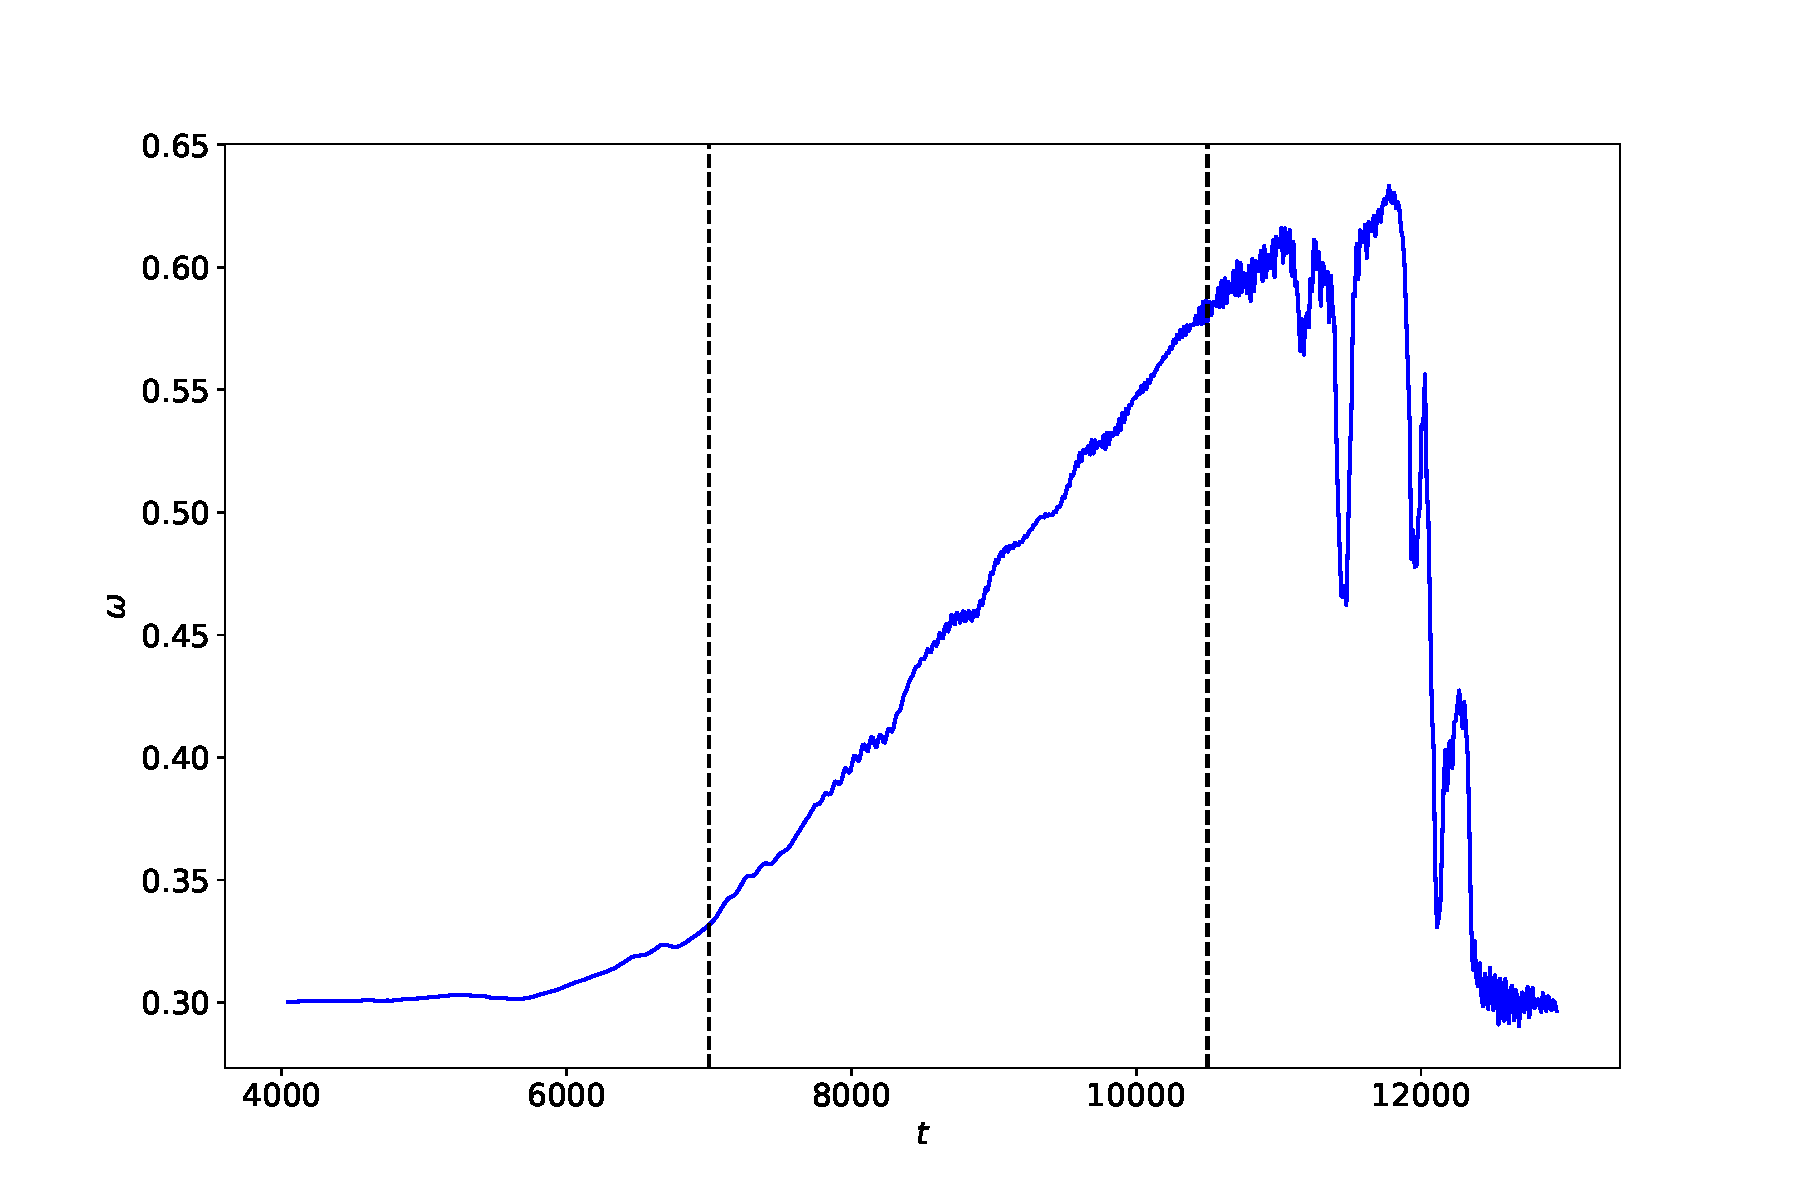
\includegraphics[width=0.7\textwidth]{Frequency_idspersion.pdf}
  \caption{Frequency idspersion}
\end{figure}
우리는 아래의 식에 각각의 데이터를 넣어 계수 $\beta_{1}$과 $\beta_{2}$ 를 구해야 한다. 
\begin{equation}
\begin{split}
\left\{
\begin{array}{r}
y_1 = f(x_1, \boldsymbol{\beta}) \equiv \beta_{1} + \beta_{2}x_1 \\
y_2 = f(x_2, \boldsymbol{\beta}) \equiv \beta_{1} + \beta_{2}x_2 \\
y_3 = f(x_3, \boldsymbol{\beta}) \equiv \beta_{1} + \beta_{2}x_3 \\
\vdots  \\
y_N = f(x_N, \boldsymbol{\beta}) \equiv \beta_{1} + \beta_{2}x_N \\
\end{array}
\right.
\end{split}
\end{equation}
이때 우리가 구하고자 하는 것은, 이 점선 사이에서 Linear한 값을 뜨는 부분의 데이터를 통해, Linear Model Fitting을 하여 직선을 그리고, 그것의 기울기를 그리는 것이다. 그러기 위해서는, 앞서 배운 최소 제곱법을 사용한다. 먼저 함수를 불러오면,
\begin{lstlisting}[language=Python]
def least_squares(X, y):
    XT = np.transpose(X)
    return la.solve(XT @ X, XT @ y)
\end{lstlisting}
이 함수를 사용하려면 Parameter 값으로, N $\times$ M 사이즈의 행렬(A라고 하자)이 필요하고, 또한, N크기의 열 벡터가 필요하다. 또한 우리가 그릴 그래프는 선형 모델이기 때문에, 행렬 A의 첫번째 열은 1로 존재하면 된다. 
\begin{equation}
\begin{split}
\mathbf X
=
\left(
\begin{matrix}
\phi_1(x_1) & \phi_2(x_1) \\
\phi_1(x_2) & \phi_2(x_2) \\
\phi_1(x_3) & \phi_2(x_3) \\
\phi_1(x_4) & \phi_2(x_4) \\
\vdots & \vdots \\
\phi_1(x_N) & \phi_2(x_N) \\
\end{matrix}
\right)
=
\left(
\begin{matrix}
1 & x_1 \\
1 & x_2 \\
1 & x_3 \\
1 & x_4 \\
\vdots & \vdots \\
1 & x_N \\
\end{matrix}
\right)
,\qquad
\mathbf y
=
\left(
\begin{matrix}
y_1 \\
y_2 \\
y_3 \\
y_4 \\
\vdots \\
y_N \\
\end{matrix}
\right)
\end{split}
\end{equation}
위 공식에 맞추기 위해 $x_1$,...,$x_N$ 의 데이터와 $y_1$,...,$y_N$를 얻기 위해 dataframe에서 우리가 원하는 7000과 10500사이의 값만 필터링 되도록 맞춰주고, 이를 least squares 를 불러와 함수의 계수 $\beta_1$과 $\beta_2$ 를 구해준다. 이때 우리가 구하고자 하는 $d\omega/dt$는 곧 $\beta_2$ 값이다. 이를 파이썬으로 구현하면 다음과 같다.

\begin{lstlisting}[language=Python]
In:
#import data
df = pd.read_csv('frequency_dispersion.tsv', sep = '\t')

#filter
is_min = df['time'] > 7000 
is_max = df['time'] < 10500
df = df[is_min & is_max]



#import data in xi, yi
xi = list(df['time'])
yi = list(df['        \"freq\"']) 

# define matrices, X and y
X = np.vstack([
    np.ones(len(xi)),
    xi
]).T
Y = yi

# find least-squares solution
b1, b2 = least_squares(X, Y)
print(f"""
beta_1 = {b1}, dw / dt = {b2}
""")


# draw
plt.figure(figsize=[12, 10])
ax = plt.subplot()

plt.plot(xi, yi, "-r", markeredgecolor="k",
         label="frequency_dispersion.tsv")

xs = np.linspace(7000, 10500, 100)
ys = b1 + b2*xs
plt.plot(xs, ys, "-b", label="Least-squares fit")

plt.title('Linear in the time 7000 < $t$ < 10500]',fontsize = 20)
plt.xlim([7000, 10500])
plt.ylim([0.30, 0.7])
plt.grid()
plt.legend()
plt.xlabel("$t$")
plt.ylabel("$\omega$")

plt.show()

Out:
beta_1 = -0.18958694289430608, dw / dt = 7.36600470144523e-05
\end{lstlisting}
\subsection{Execution and Assessment}
\begin{figure}[!ht]
  \centering
  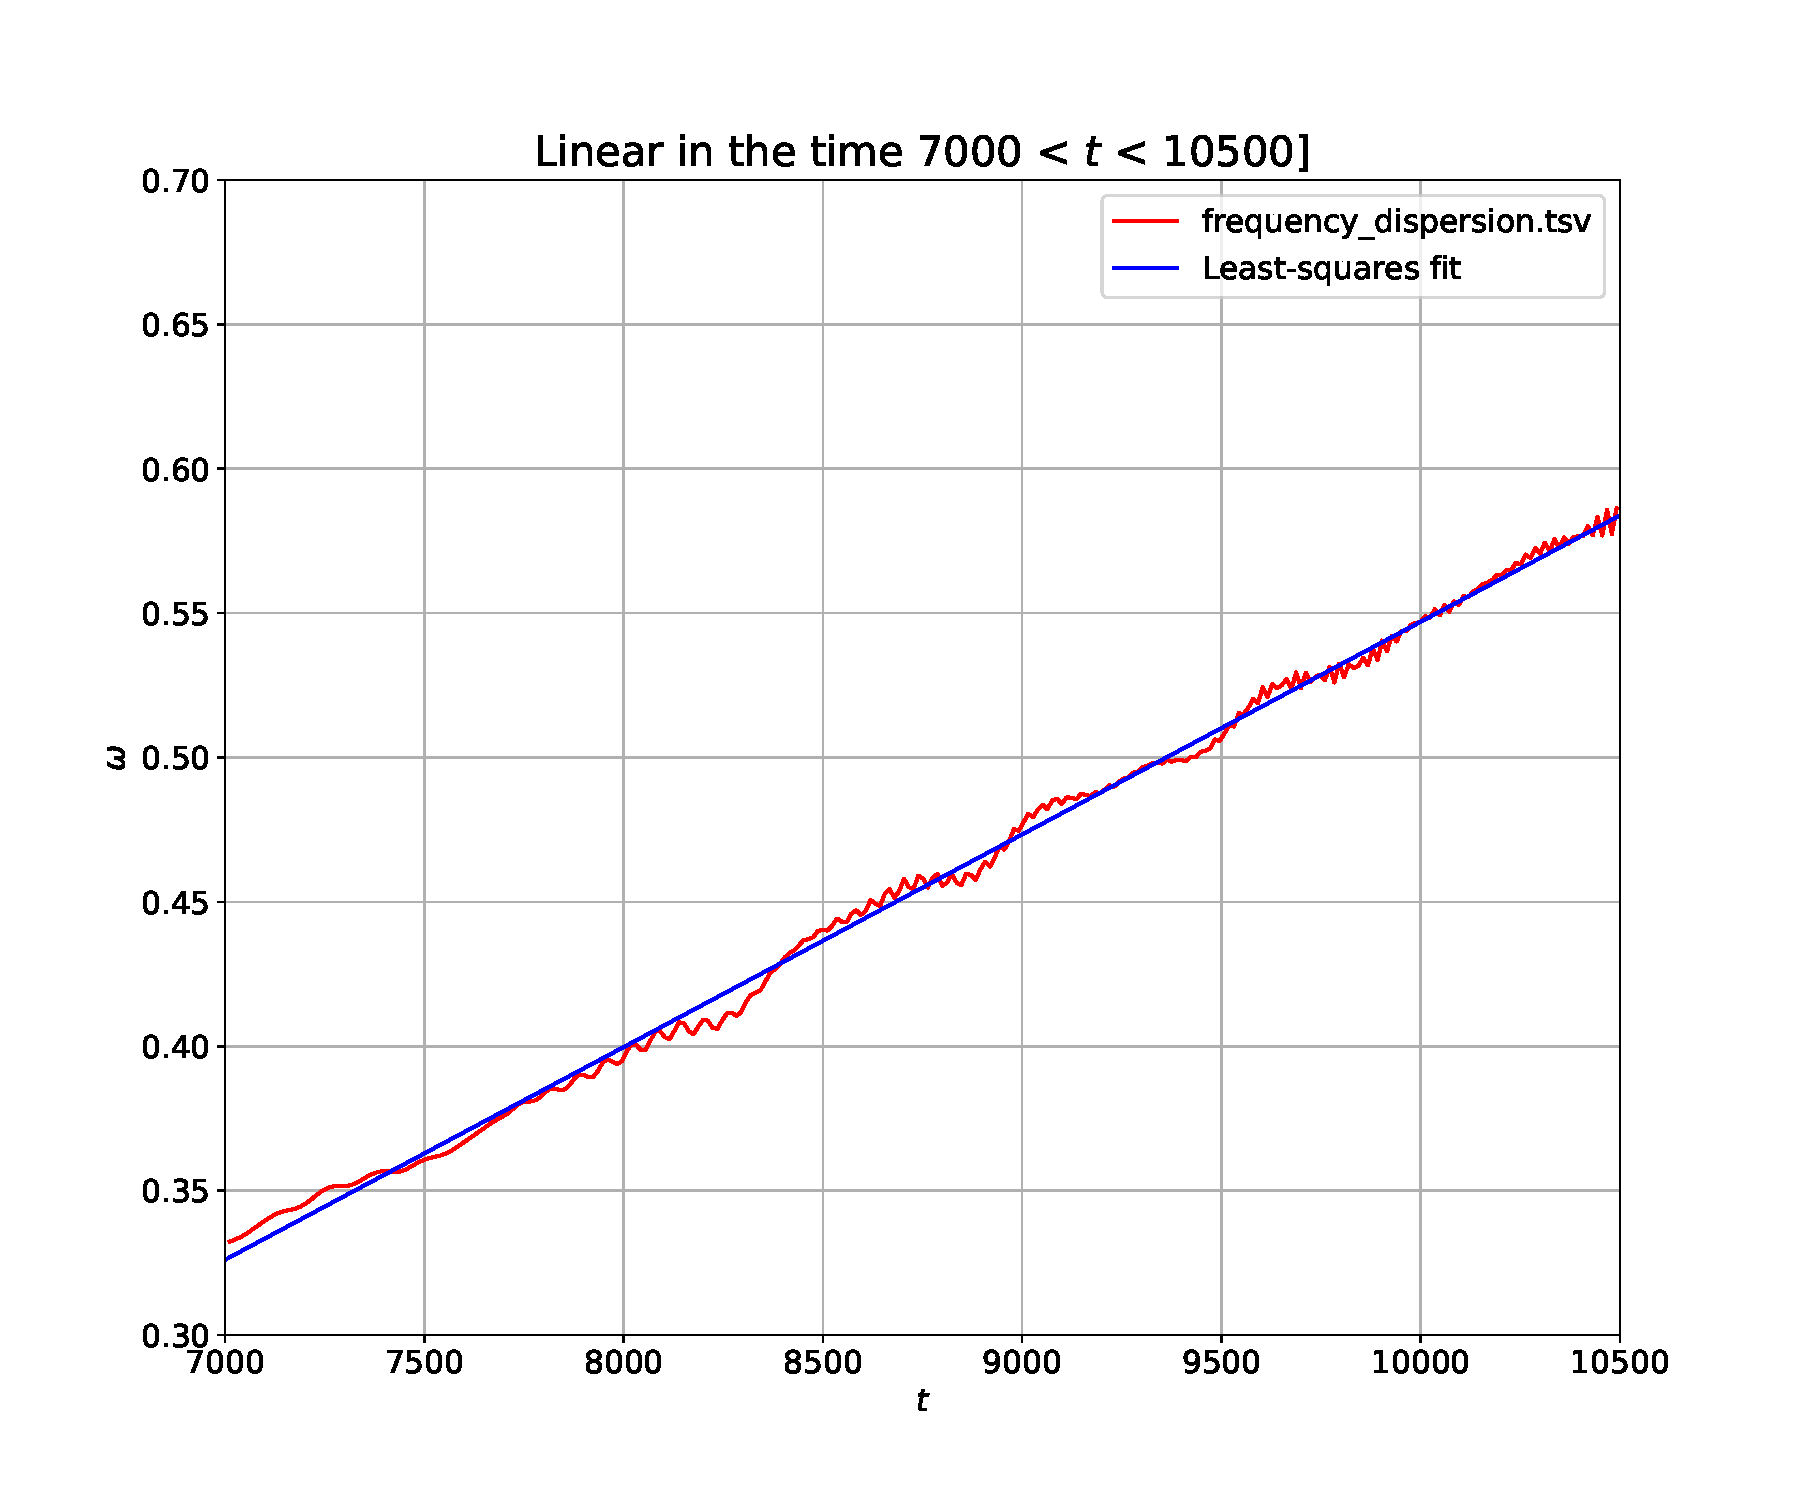
\includegraphics[width=0.7\textwidth]{Linear_in_the_time.pdf}
  \caption{Linear-Least Squares fit}
\end{figure}
우리가 구하고자 한 모습과 동일하게, 선형적인 양상을 띄는 것을 볼 수 있고, 이것의 기울기 또한, 7.36600470144523e-05 라는 것을 알 수 있다.
\pagebreak









\section{Runge's Phenomenon}
\subsection{Problem Recognition} 
Runge's Phenomenon은 등간격 보간점 집합에 대해 고차항 다항식과 다항식 보간을 사용할 때 발생하는 간격의 가장자리에서의 진동 문제이다. 따라서, 일반적인 관점에서 동일한 간격의 격자점은 고차 다항식 적합에 적합하지 않는 것을 알려주는 현상이다.

\begin{enumerate}
    \item  다음의 함수를 고려하자
    \begin{equation}
    u(x) = \frac{1}{1 + 16x^2}
    \end{equation}
    이때 우리는 N = 16일때, $v_j = u(x_j)$를 만족하는 함수를 사용할 것이다. 
    \begin{equation}
    x_j = -1 + 2\frac{j}{N}
    ,\qquad
    j = 0, 1, \dots, N
    \end{equation}
    이때, 이 N차의 다항식에 대해 Polynomial Fitting 하여 $P_N(x)$를 각각의 데이터 $(x_j, v_j)$를 이용하여 구한다. 이때 구해진 $P_N(x)$와 $u(x_j)$를 비교해본다.
     \item Runge's Phenomenon를 대처하기 위해서는, 가장 간단한 예로 Chebyshev points라고 불리는, 불규칙한 간격의 해를 사용하면 된다. 이는 다음과 같다.
         \begin{equation}
     x_j = \cos\left(\frac{j\pi}{N}\right)
    ,\qquad
    j = 0, 1, \dots, N
        \end{equation}
        	이때, $(x_j, v_j)$을 통해 Polynomial Fitting 한 함수를 $Q_N(x)$라고 정의하고, $Q_N(x)$와 $u(x_j)$를 비교해본다.
    
\end{enumerate}
\subsection{Development of a solution} 
먼저 이 문제를 1, 2의 방식에 맞추어 먼저 함수를 그려주고, 그렇게 구한 점들을 N차 Polynomial Fitting 방식을 통해, n+1 지점을 통과하는 n차 다항식을 찾아주어 함수를 그래프로 그려내면 된다. 다항식을 찾기 위해, 우리는 앞서 배운 poly fit과 poly val 함수를 불러 사용할 것이다. 따라서 먼저 poly fit을 사용하기 위한 xs, ys 점들의 리스트를 정해주어야 한다. 우리는 그 점들을 각각의 경우에 대한 $x_j$에 대한 식을 대입하고, 그로 인해 구해지는 계수를 poly val을 통하여 다항식을 유추한다. 그리고 임의의 x 값을 linspace로 지정해준 뒤, 각각의 경우에 대해 $v_j$함수와 $P_N(x)$, $Q_N(x)$ 함수를 비교해준다.

\begin{lstlisting}[language=Python]
In:
N = 16
#1.
xi = [-1 + (x/8) for x in range(0, N+1)]
yi = [1 / (1 + (16 * x**2)) for x in xi]

# 1-degree polynomial (i.e., line) fitting
coefs = poly_fit(xi, yi)


# define the grid points to display the fit polynomial
x = np.linspace(-1, 1, 100)
p = poly_val(coefs, x)

x_exact = x
y_exact = [1 / (1 + 16 * x ** 2) for x in x_exact]

#figure size
plt.figure(figsize = (10, 10))

#draw 1 figure
plt.subplot(2,1,1)
plt.xlim(-1, 1)
plt.ylim(0, 1)
plt.plot(x_exact, y_exact, "-y", label="$v_{j}(x)$")
plt.plot(x, p, "-b", x, p, ".r", label="$P_{N}(x)$") #, label='$P_{n}(x) dot$')
plt.legend()
plt.grid()
plt.ylabel("$v_{j}$")

#2.
xj = [np.cos((x * np.pi) / N) for x in range(0, N+1)]
yj = [1 / (1 + (16 * x**2)) for x in xj]

# 1-degree polynomial (i.e., line) fitting
coefs = poly_fit(xj, yj)

# define the grid points to display the fit polynomial
x = np.linspace(-1, 1, 100)
p = poly_val(coefs, x)

#draw 2 figure
plt.subplot(2,1,2)
plt.plot(x_exact, y_exact, "-y", label="$v_{j}(x)$")
plt.plot(x, p, "-b", x, p, ".r" , label="$Q_{N}(x)$")
plt.grid()
plt.legend()

plt.xlabel("$x_{j}$")
plt.ylabel("$v_{j}$")
plt.savefig('Runge_Phenomenon.pdf')
\end{lstlisting}

\subsection{Execution and Assessment}
예상했던대로, $x$를 규칙적인 동일한 간격의 격자점은 고차 다항식에 적합하지 않는 것을 볼 수 있다. 다른 고차 함수를 넣더라도, 동일한 간격의 $x_j$를 사용하여 Linear fitting을 진행하면, 마찬가지로 가장자리 점에는 진동하는 모습을 볼 수 있다. 이것으로 우리는, 함수가 고차항에 가까우면, 동일한 간격을 주지 않는 예를 들어, Chebyshev points 인 경우, 이를 막을 수 있다.  이 경우,

\begin{figure}[!ht]
  \centering
  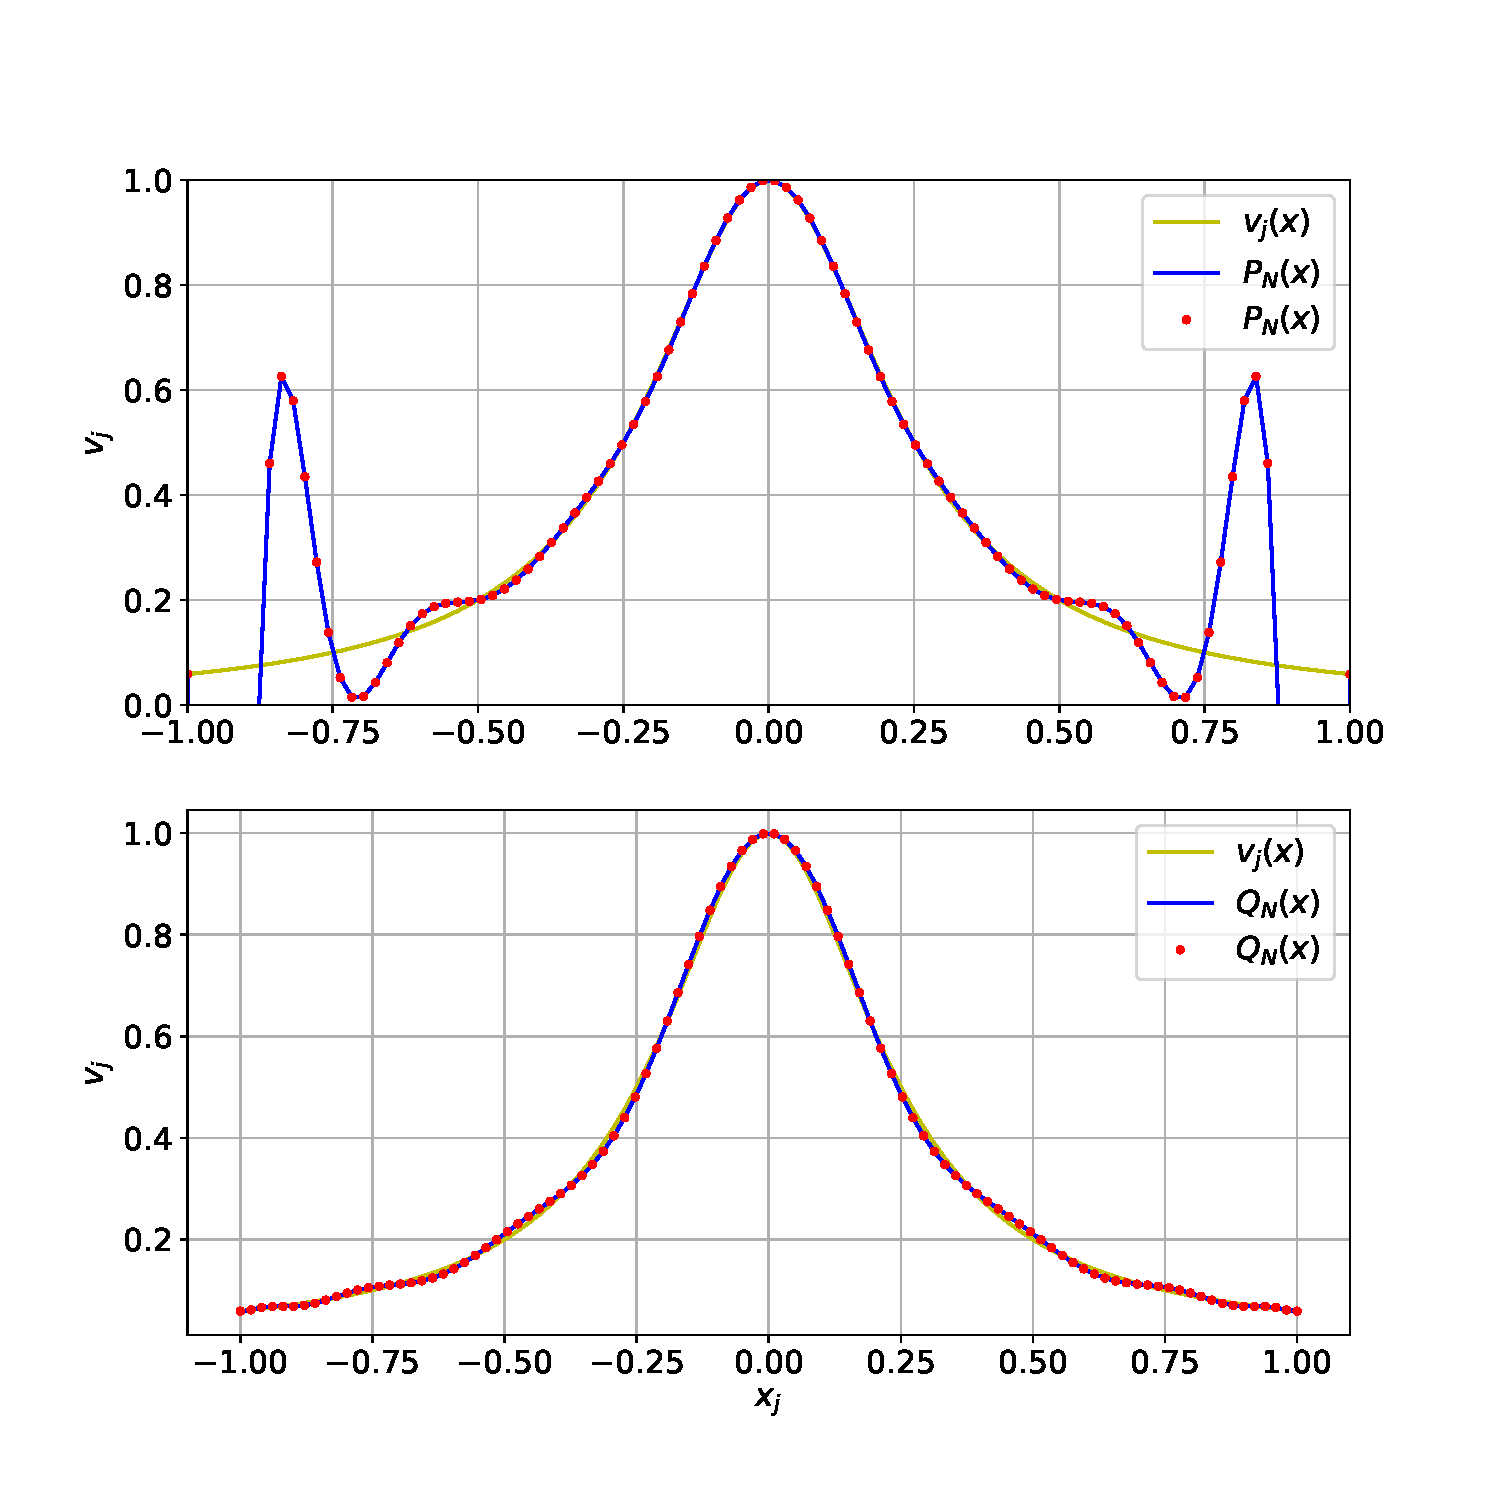
\includegraphics[width=1\textwidth]{Runge_Phenomenon.pdf}
  \caption{Runge's Phenomenon}
\end{figure}
\pagebreak

하지만 모든 경우에 있어서 그런 조건을 만족함에도 풀 수 있는 것은 아니다. 

바로 Singular Matrix 오류가 발생하기 때문이다. 우리가 다항식의 계수를 풀어 다항식 회귀 분석을 하는데, 만약에 주어진 점에 대해서, 









\section{Two-point BVPs}
\subsection{Problem Recognition} 
다음 문제, $u_{xx} = e^{4x}$ 를 $-1 < x < 1$ 에서 아래의 초기 조건에 따라 풀어보어야 한다.
\begin{enumerate}
    \item  Set 1: 
    \begin{equation}
    u(-1) = 0,
    \quad
    u( 1) = 0
        \end{equation}
        \item  Set 2:
            \begin{equation}
            u(-1) = 0
    ,\quad
    u( 1) = 1
                    \end{equation}
            \item  Set 3:
                        \begin{equation}
                        u(-1) = 1
    ,\quad
    u( 1) = 0
                                \end{equation}
                \item  Set 4:
                            \begin{equation}
                            u(-1) = 1
    ,\quad
    u( 1) = 1
                                    \end{equation}
    
\end{enumerate}
\subsection{Development of a solution} 
미분 방정식에서 경계 조건이라는 추가 제약이 존재하는 미분 방정식을 풀어야 한다. 따라서 먼저 선행해서 배운 finite diff 2nd 함수를 불러와 이차 미분 방정식을 풀어줄 것이다. 
\begin{lstlisting}[language=Python]
def finite_diff_2nd(N):
    """Create a N-by-N matrix corresponding to the second-order central difference formula.
    
    The returned matrix must be divided by h^2.
    """
    
    assert N > 2, "at least three points are required"
    
    main_diag = -2 * np.eye(N)
    down_diag = np.diagflat(np.ones(N - 1), -1)
    return main_diag + down_diag + down_diag.T
    \end{lstlisting}
이때 우리는 우변의 값이 무엇인지를 제대로 확인해 볼 필요가 있다. 우리가 문제에서 풀고자 한 함수는, $u_{xx} = e^{4x}$이다. 따라서, 우변 값은 $e^{4x}$이고 이는 곧, 우리가 구하고자 하는 wj에 해당하는 값이다. 그리고 각각에 대한 초기 값은, a, b에 해당하는 값이므로 wj의 첫번째 인덱스 값은 -1을 넣었을시 값이 되고, 이는 Set에 정해져 있는 $u(-1)$값을 뜻하고, x의 마지막 값, 1은 wj의 마지막 인덱스 값으로 $u(1)$를 의미한다. 각각의 경우에 대해 함수를 그려주면, 다음과 같다. 그리고 우리는 이것을 전에 다뤘던 Predictor-corrector Method 에서 다룬 heun의 방식을 통하여 해를 근사적으로 구하고, 대략적으로 적합한지를 고려해 볼 것이다.

\begin{lstlisting}[language=Python]
#Root Finding solution
def F(t, Y): # F = [v, -g], Y = [x, v]
    F = [Y[1], np.exp(4*t)]
    return np.array(F)

# boundary values
boundary_values = [0, 0], [0, 1], [1, 0], [1, 1]

# uniformly discretized domain
N  = 100
xj = np.linspace(-1, 1, N)
h  = xj[1] - xj[0]

# right-hand side
wj = np.exp(xj*4)

# finite difference matrix w/ boundary conditions imposed
D2 = finite_diff_2nd(N) / h**2

# 1. decimate the first and last rows
D2[ 0, :] *= 0
D2[-1, :] *= 0

# 2. replace 1,1 and N,N components with 1
D2[ 0,  0] = 1
D2[-1, -1] = 1
plt.figure(figsize = (15, 9))

for i, x in enumerate(boundary_values):
    a, b = x
    n = i + 1
    wj[0], wj[-1] = a, b # this is where the boundary values go to


    # solve linear equations
    phij = la.solve(D2, wj)

    # draw
    plt.subplot(2, 2, n)
    plt.plot(xj     , phij   , "--r", label="$\\phi_j$")
    
    t    = np.linspace(-1, 1, 100)
    Y_0  = np.array([0, 0])
    x, v = zip(*heun_ode(F, Y_0, t))
    plt.plot(t, x, ':k', label = 'Root Finding Solution')  
    plt.title(f"boundary value is u({-1}) = {a}, u({1}) = {b}")
    #x, y label
    if n == 3 or n == 4:
        plt.xlabel("$x$")
    if n == 1 or n == 3:
        plt.ylabel("$u$")
    plt.grid()
    plt.legend()
    #plt.title(f"{n}th eigen mode: $k_{n} = {k:.2f}$")
plt.savefig("Two-point_BPS.pdf")

if t[-1] == 1:
            print(f"Heon's Solution : u({1}) = {x[-1]}" )
            
Out:
Heon's Solution : u(1) = 3.400221185772245


\end{lstlisting}
\pagebreak
\subsection{Execution and Assessment}
\begin{figure}[!ht]
  \centering
  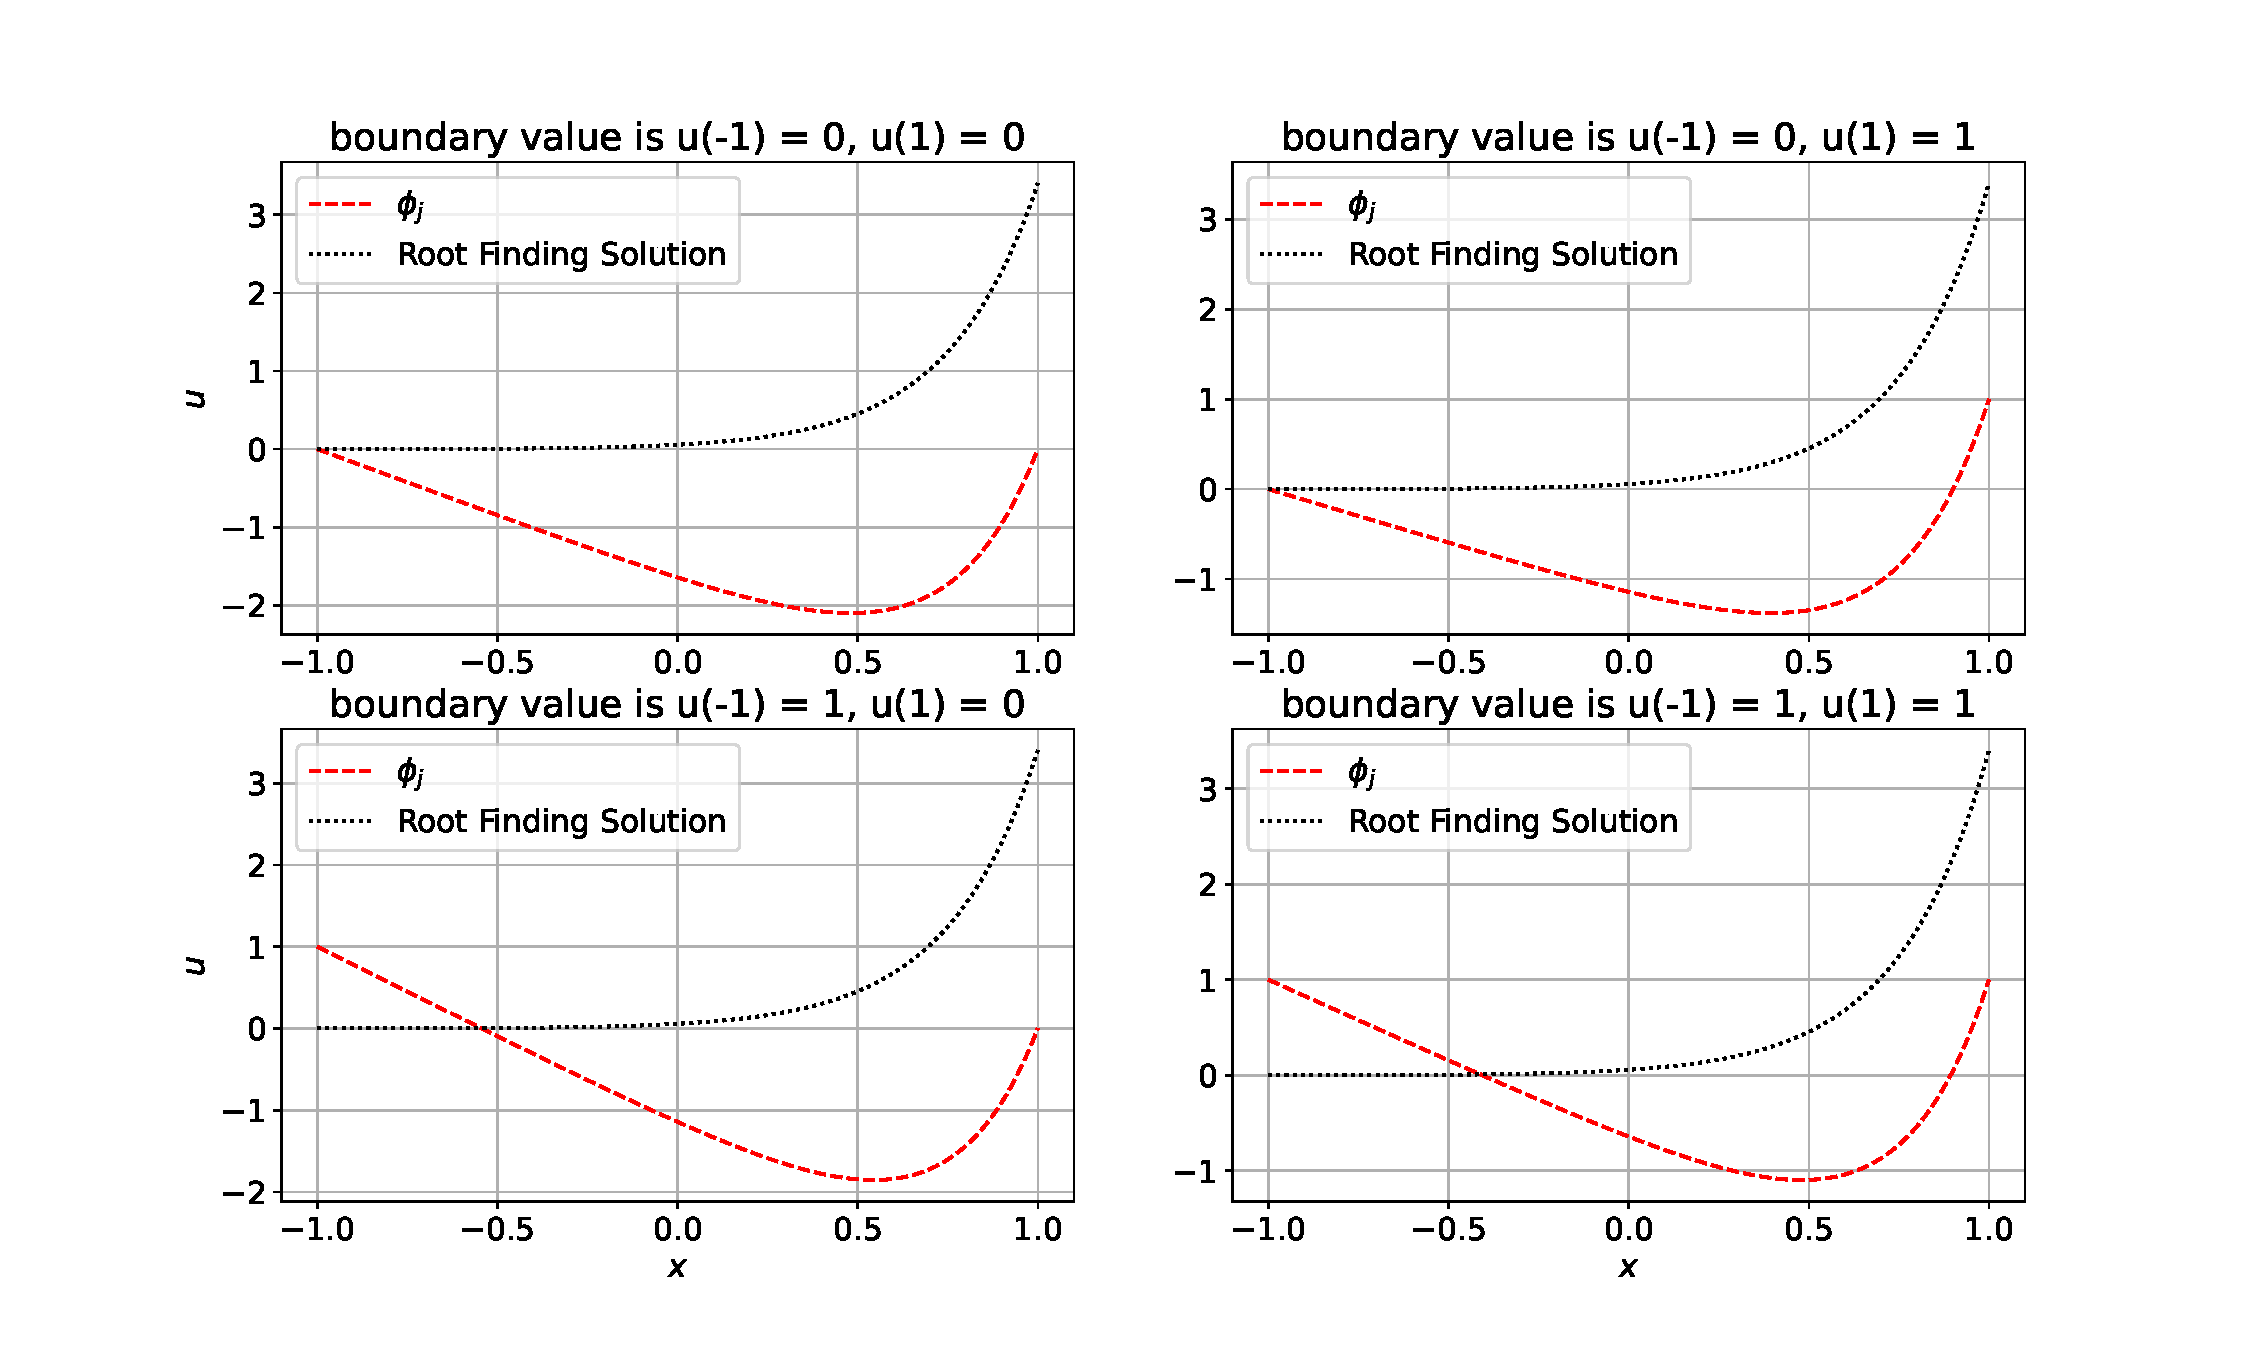
\includegraphics[width=1\textwidth]{Two-point_BPS.pdf}
  \caption{Two-point BVPs}
\end{figure}

그래프 모양을 잘 살펴보면, 사실 실제 근과 비슷하게 만들어진 것을 볼 수 있다. 따라서 만약 우리가 원하는 해에 근사한 경계값만 알게 된다면, 더 정확도가 높은 값을 유추할 수 있다. 예를 들어, x = 0 을 고정으로 두고, 만약 y값을 적절하게 다시 그리게 되면,



\begin{lstlisting}[language=Python]
# Root Finding definition
def F(t, Y): # F = [v, -g], Y = [x, v]
    F = [Y[1], np.exp(4*t)]
    return np.array(F)

# boundary values
boundary_values = [0, 2.5], [0, 3], [0, 3.5], [0, 3.388]

# uniformly discretized domain
N  = 100
xj = np.linspace(-1, 1, N)
h  = xj[1] - xj[0]

# right-hand side
wj = np.exp(xj*4)

# finite difference matrix w/ boundary conditions imposed
D2 = finite_diff_2nd(N) / h**2

# 1. decimate the first and last rows
D2[ 0, :] *= 0
D2[-1, :] *= 0

# 2. replace 1,1 and N,N components with 1
D2[ 0,  0] = 1
D2[-1, -1] = 1
plt.figure(figsize = (15, 9))

for i, x in enumerate(boundary_values):
    a, b = x
    n = i + 1
    wj[0], wj[-1] = a, b # this is where the boundary values go to


    # solve linear equations
    phij = la.solve(D2, wj)

    # draw BVPs Solution
    plt.subplot(2, 2, n)
    plt.plot(xj     , phij   , "--r", label="$\\phi_j$")
    
    # draw Heun_ode Root Finding solution 
    t    = np.linspace(-1, 1, 100)
    Y_0  = np.array([0, 0])
    x, v = zip(*heun_ode(F, Y_0, t))
    plt.plot(t, x, ':k', label = 'Root Finding Solution')  
    plt.title(f"boundary value is u({-1}) = {a}, u({1}) = {b}")
    # x, y label
    if n == 3 or n == 4:
        plt.xlabel("$x$")
    if n == 1 or n == 3:
        plt.ylabel("$u$")
    plt.grid()
    plt.legend()
plt.savefig("Two-point_BPS2.pdf")

if t[-1] == 1:
            print(f"Heon's Solution : u({1}) = {x[-1]}" )
            
Out:
Heon's Solution : u(1) = 3.400221185772245

\end{lstlisting}

\begin{figure}[!ht]
  \centering
  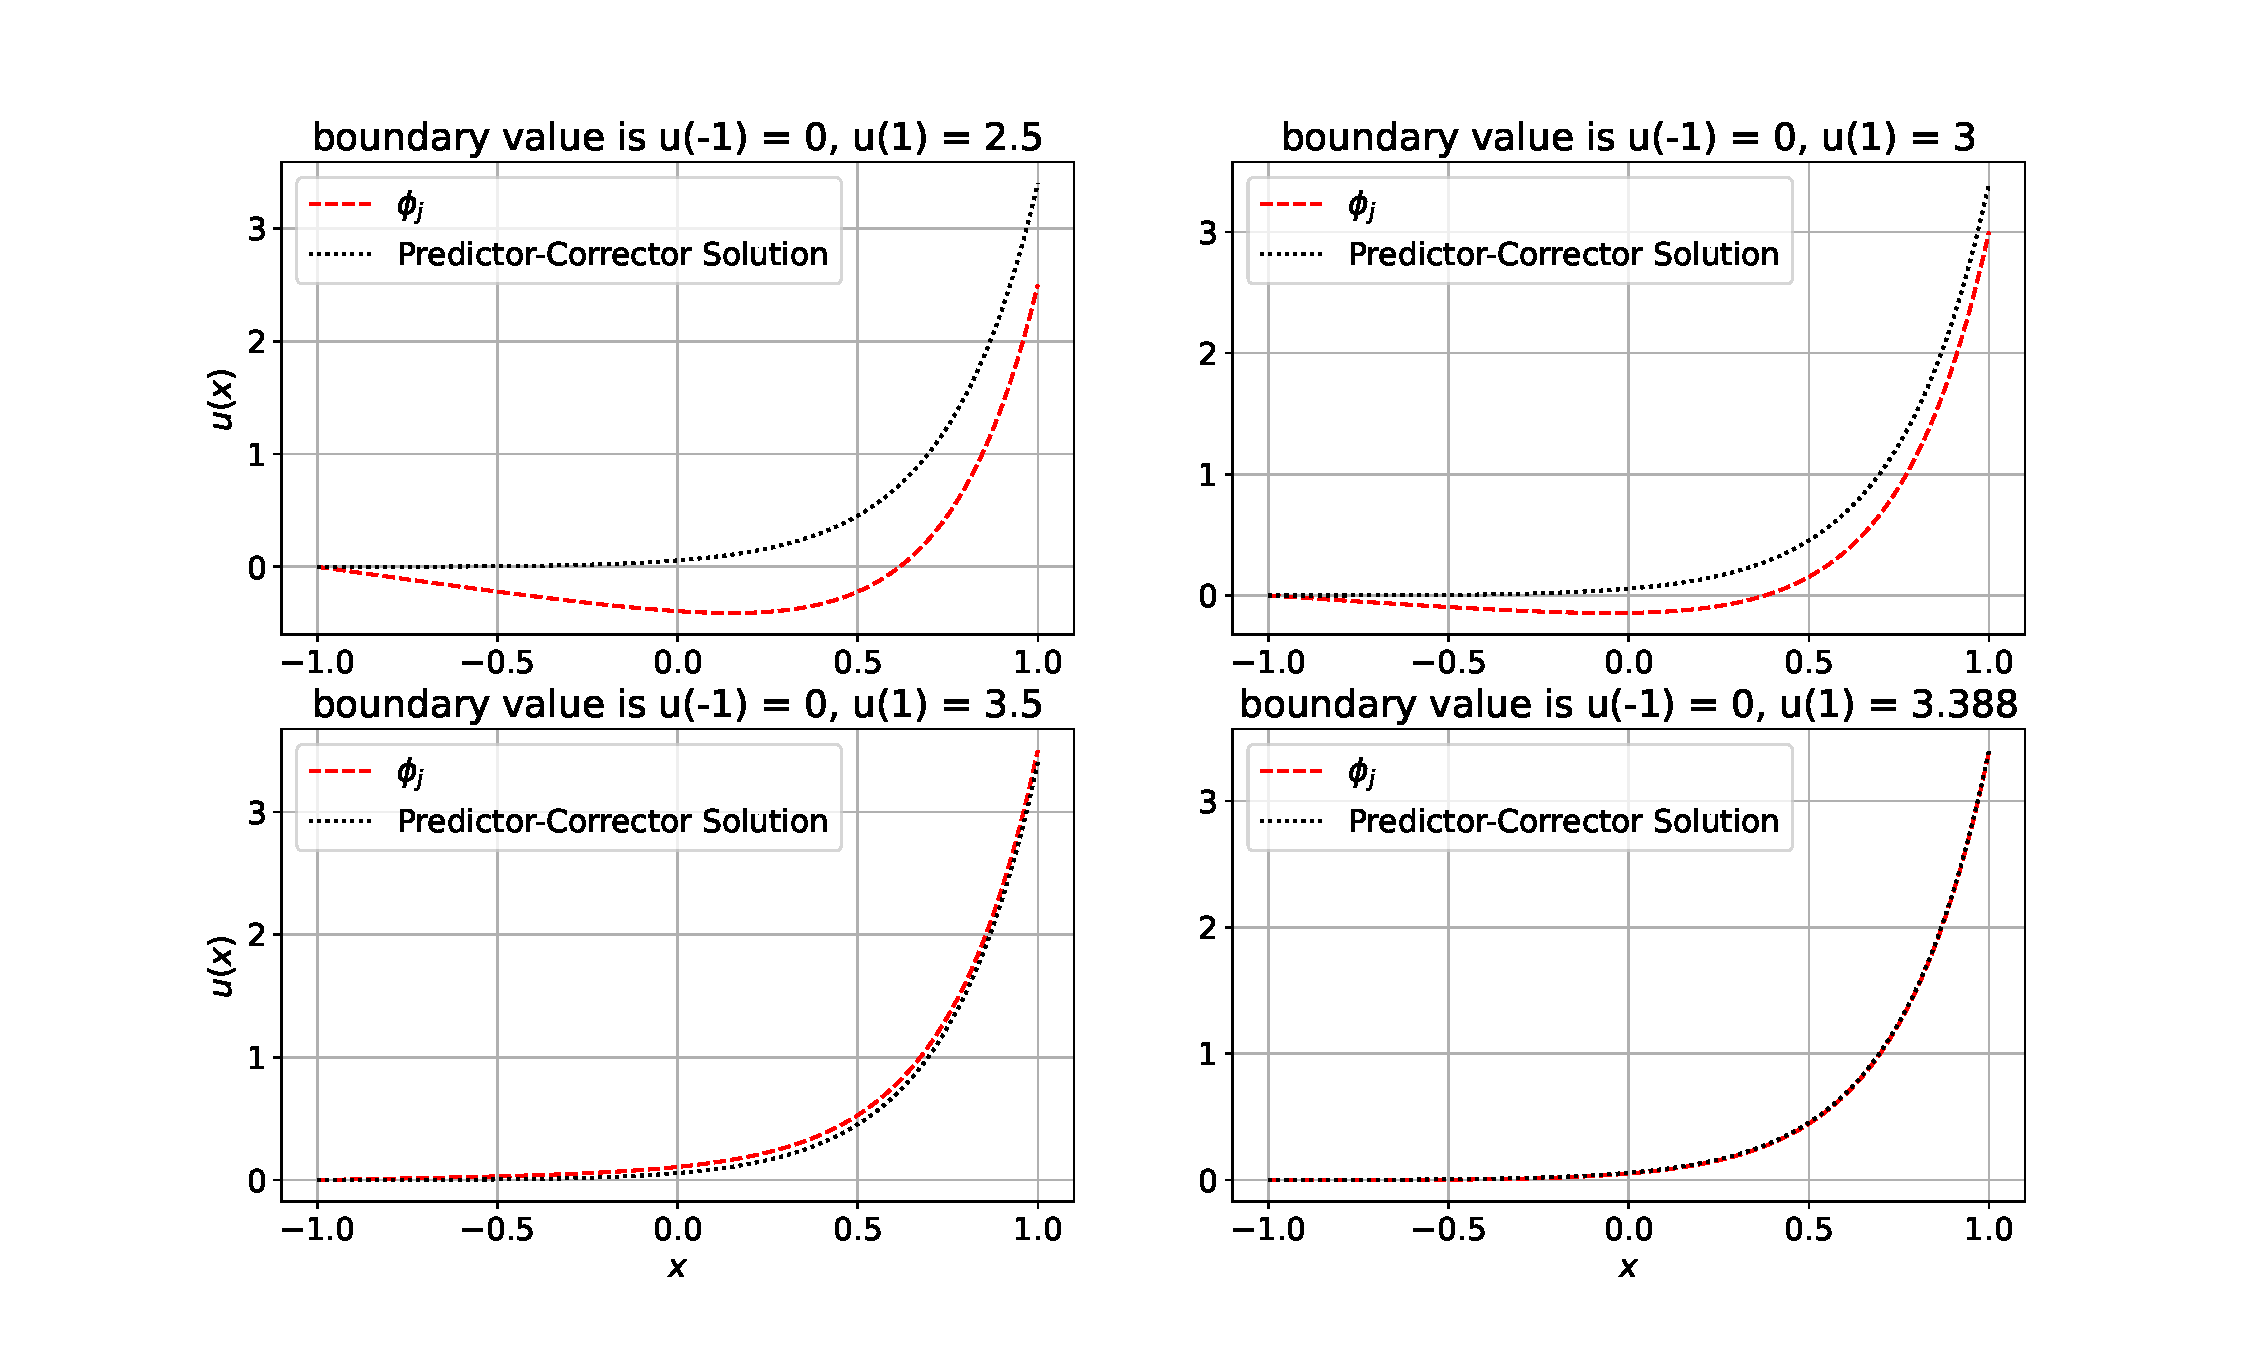
\includegraphics[width=1\textwidth]{Two-point_BPS2.pdf}
  \caption{Two-point BVPs}
\end{figure}
우리가 Heon의 방법으로 구한 해와 잘 맞아 떨어지는 것을 확인해볼 수 있다. 그렇다면 왜 초기값이 큰 기여를 하는 걸까 고민을 해볼 필요가 있다. 
\begin{equation}
\begin{split}
\left(
\begin{matrix}
\color{blue}{0} \\
w_{  2} \\
\vdots  \\
w_{N-1} \\
\color{red}{0} \\
\end{matrix}
\right)
=
\left(
\begin{matrix}
\color{blue}{
 1}           &                &               &                &               \\
\frac{1}{h^2} & -\frac{2}{h^2} & \frac{1}{h^2} &                &               \\
              &     \ddots     &    \ddots     &     \ddots     &               \\
              &                & \frac{1}{h^2} & -\frac{2}{h^2} & \frac{1}{h^2} \\
              &                &               &                & \color{red}{1} \\
\end{matrix}
\right)
\left(
\begin{matrix}
\color{blue}{u_{1}} \\
u_{  2} \\
\vdots  \\
u_{N-1} \\
\color{red}{u_{N}} \\
\end{matrix}
\right)
\end{split}
\end{equation}
BPV에서 초기값과 마지막 값을 정하는것은 우리가 문제에 주어져있는 $\omega$행렬의 첫번째 행과 마지막 행이다. 이것은 그것에 대응하는  $u(1)$ 과  $u(-1)$ 값을 넣으면 나오는 우리가 구하고자 하는 $u$의 실제 값이다.  임의의 n차 선형 미분방정식의 해에는 n개의 독립적인 임의의 상수가 포함된다. 미분방정식의 모든 해는 상수들이 특별한 값을 가지도록 하여 얻게 되므로, 따라서, 초기값에 따라서 나머지 상수부분, 즉 우리의 문제에 해당하는 상수를 포함한 방정식은 $ax + b$에서 a, b를 결정짓게 된다. 따라서 우리가 경계값을 어떻게 지정하느냐에 따라서 함수 전체의 값에 독립적으로 함수값을 더해주게 되므로, 모양은 같지만 기울어지는 모습을 볼 수 있는 것이다. 우리는 이 a, b값을 실제로 구해볼 수 있는데,  우리가 위의 식을 손으로 풀게되면, 일반해는 $\frac{e^{4x}}{16} + ax + b$이다. 만약 $u(1)$ 과  $u(-1)$가 각각 0이라면, $a = b + \frac {e^{-4}}{16}, b = -(\frac {e^{-4}}{32} + \frac {e^{4}}{32})$이라는 것을 쉽게 손으로 풀 수 있다. 그것을 대입하여 exact solution이라고 두고 그래프를 그리게 되면,

\begin{lstlisting}[language=Python]
# boundary values
a, b = 0, 0

N  = 100
xj = np.linspace(-1, 1, N)
h  = xj[1] - xj[0]

# right-hand side
wj = np.exp(4*x)
wj[0], wj[-1] = a, b # this is where the boundary values go to

D2 = finite_diff_2nd(N) / h**2
D2[ 0, :] *= 0
D2[-1, :] *= 0

D2[ 0,  0] = 1
D2[-1, -1] = 1
# solve linear equations
phij = la.solve(D2, wj)

# draw

plt.figure(figsize = (12,8))

plt.plot(xj     , phij   , "--r", label="$BVP solution$")


x = np.linspace(-1, 1, 100)
plt.plot(x, -(np.exp(-4)/32 + np.exp(4)/32) +  (-(np.exp(-4)/32 + np.exp(4)/32) + np.exp(-4)/16) * x + np.exp(x * 4) / 16, ':k', label="$Exact solution$")
plt.xlabel("$x$")
plt.ylabel("$u$")
plt.grid()
plt.legend()
plt.savefig('BVPsolution_Exact.pdf')
\end{lstlisting}

\begin{figure}[!ht]
  \centering
  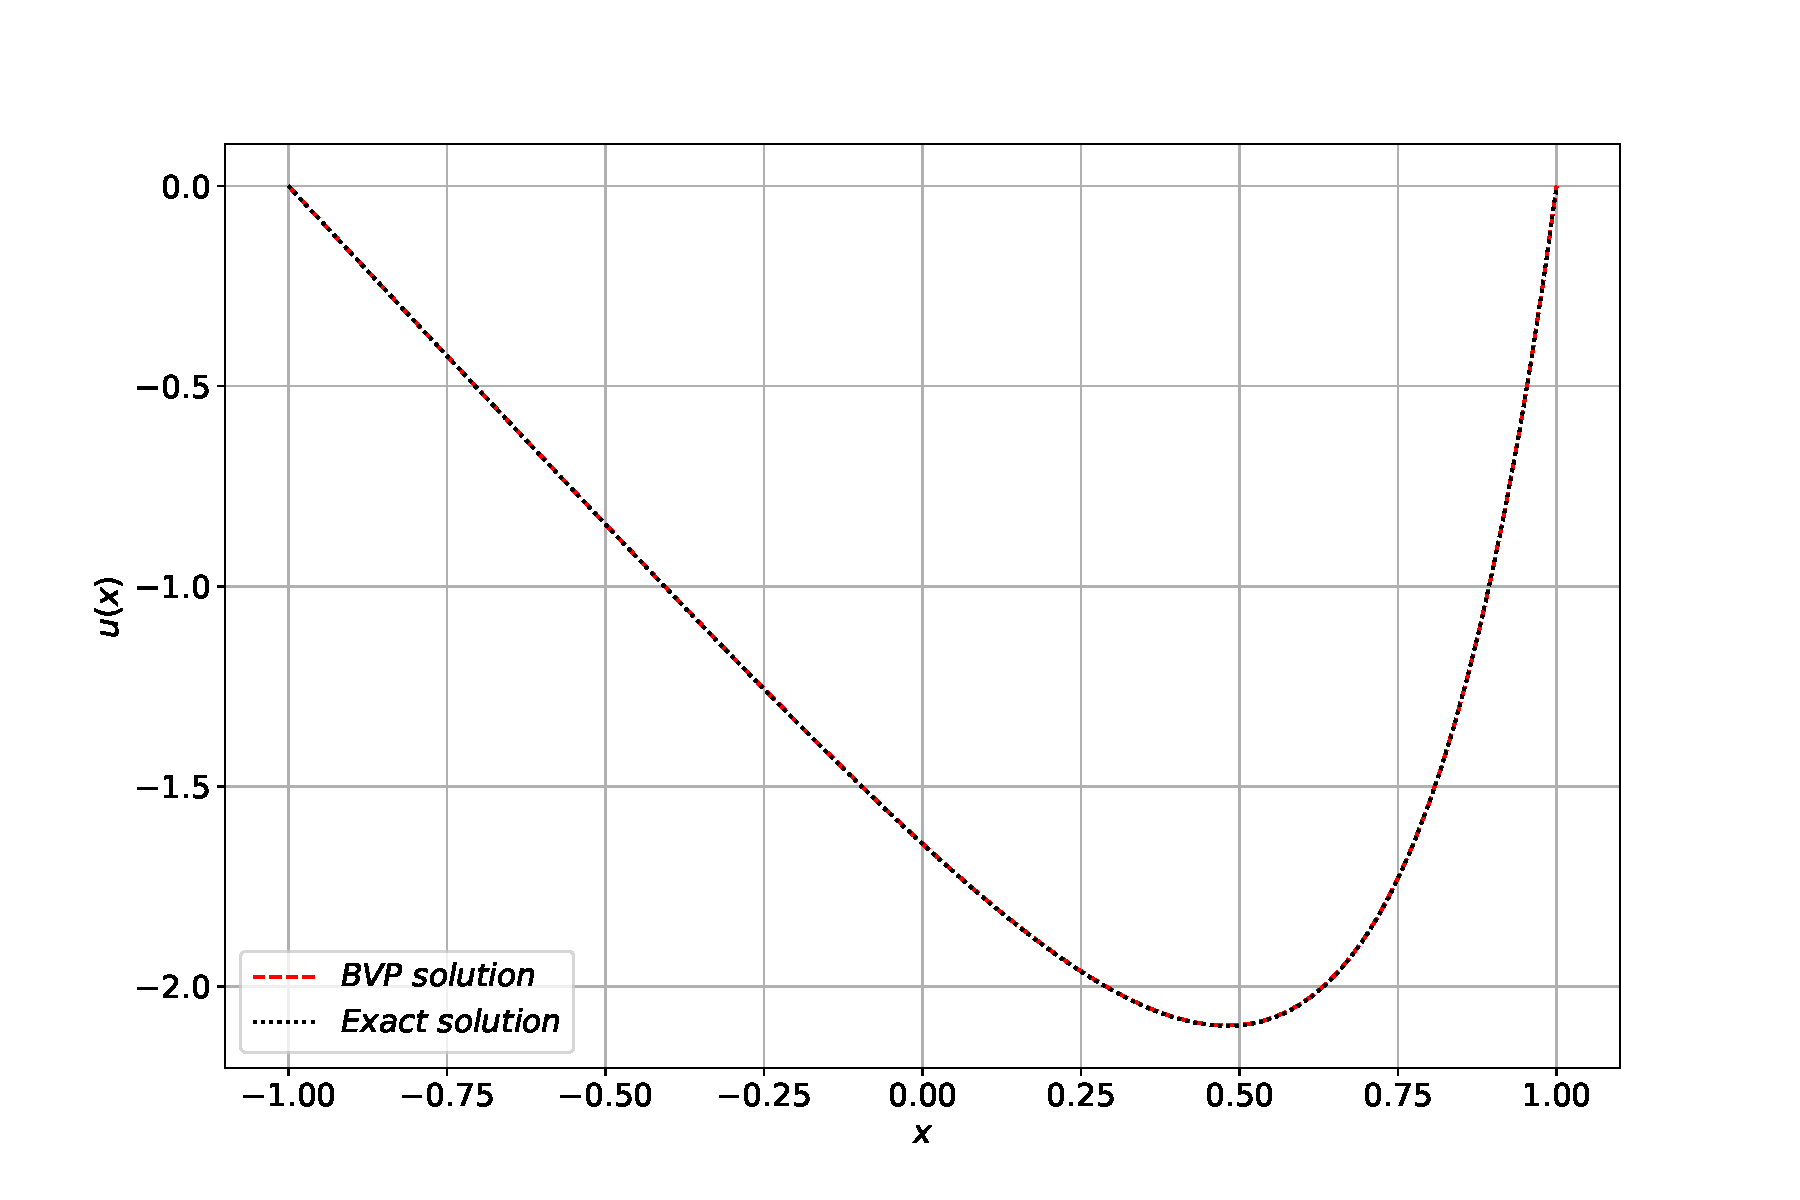
\includegraphics[width=0.8\textwidth]{BVPsolution_Exact.pdf}
  \caption{Two-point BVPs and exact solution}
\end{figure}
우리가 처음에 구한 함수와 잘 맞아 떨어지는 것을 볼 수 있다. 따라서, 이 경계값은 함수에 선형 독립적이게 함수에 일정한 비율의 크기를 빼거나 더해준다는 것도 이해할 수 있다. 그렇다면 이를 토대로 Heon으로 구한 1에서의 경계 값 $u(1) = 3.400221185772245$을 이용하여 상수 값을 계산하면, 
\begin{lstlisting}[language=Python]
# boundary values
a, b = 0, 3.400221185772245

N  = 100
xj = np.linspace(-1, 1, N)
h  = xj[1] - xj[0]

# right-hand side
wj = np.exp(4*xj)
wj[0], wj[-1] = a, b # this is where the boundary values go to

D2 = finite_diff_2nd(N) / h**2
D2[ 0, :] *= 0
D2[-1, :] *= 0

D2[ 0,  0] = 1
D2[-1, -1] = 1

# solve linear equations
phij = la.solve(D2, wj)

# draw

plt.figure(figsize = (12,8))

plt.plot(xj     , phij   , "--r", label="$BVP$ $solution$")

xj = np.linspace(-1, 1, N)
x = 3.400221185772245
b1 = x / 2 - (np.exp(-4) / 16 + np.exp(4) / 16) / 2
a1 = x + -np.exp(4)/16 - b1
plt.plot(xj, np.exp(4 * xj) / 16 + a1 * xj + b1, ':k', label="$Exact$ $solution$")
plt.xlabel("$x$")
plt.ylabel("$u(x)$")
plt.grid()
plt.legend()
plt.savefig('BVPsolution_Exact3.pdf')
\end{lstlisting}

\begin{figure}[!ht]
  \centering
  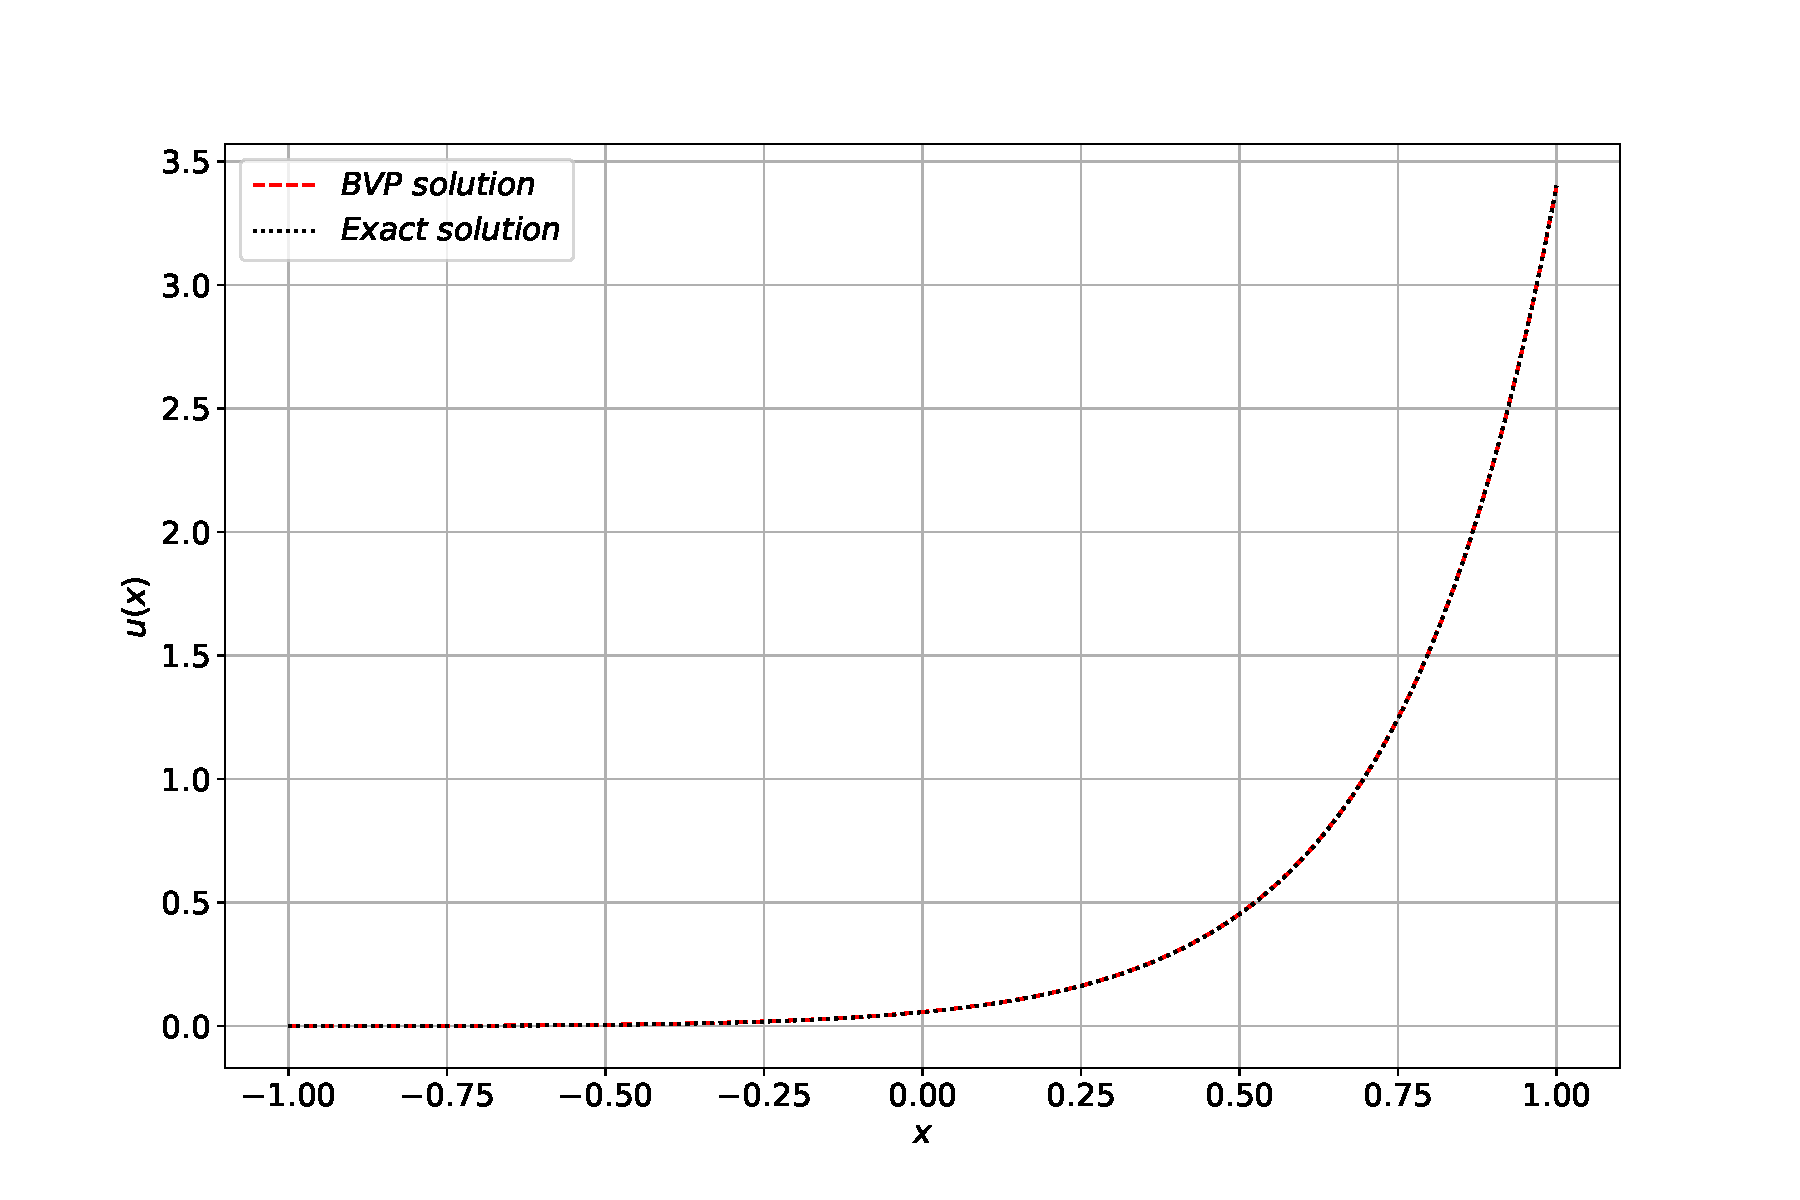
\includegraphics[width=0.8\textwidth]{BVPsolution_Exact3.pdf}
  \caption{Two-point BVPs and exact solution by $u(x) =  3.400221185772245$}
\end{figure}

\end{document}


